\section{RET - Reaktanz-Eintore}
\subsection{Reaktanzen}
	\begin{tabular}{ll ll}
		\parbox{4cm}{
			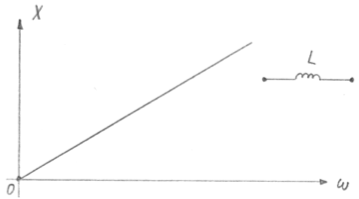
\includegraphics[width=3.5cm]{./bilder/Induktivitaet}
			}
			& \parbox{5cm}{
				\textbf{Induktivität} \\
				$\underline{Z}=j\omega L \qquad X=\omega L$\\
				$B=-\frac{1}{\omega L}$\\
				Nullstelle: $\lim\limits_{\omega \rightarrow 0} X(\omega) = 0$ \\
				Polstelle: $\lim\limits_{\omega \rightarrow \infty} X(\omega) = \infty$ \\
			}
			
			& \parbox{4cm}{
			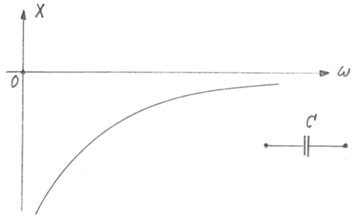
\includegraphics[width=3.5cm]{./bilder/Kapazitaet}
			}
			& \parbox{5cm}{
				\textbf{Kapazität} \\
				$\underline{Z}=\frac{1}{j\omega C}=\frac{-j}{\omega C} \qquad X=\frac{-1}{\omega C}$\\
				$B=\omega C$ \\
				Nullstelle: $\lim\limits_{\omega \rightarrow \infty} X(\omega) = 0$ \\
				Polstelle: $\lim\limits_{\omega \rightarrow 0} X(\omega) = -\infty$ \\
			}
	\end{tabular}
	
\subsection{Vorgehen bei Netzwerkanalyse}
	\begin{enumerate}{\setlength{\itemsep}{0cm}\setlength{\parsep}{0cm} \setlength{\topsep}{0cm}}
      \item Schaltung übersichtlich aufzeichenen und den Startpunkt der Addition bestimmen
      \item Frequenzverlauf der Reaktanz finden durch fortgeschrittene Addition und Inversion
      \item Inversion: $B(\omega)=\frac{-1}{X(\omega)}$ ; $Polstelle \Longleftrightarrow Nullstelle$
      \item Die so entstandenen Pole und Nullstellen, ausser 0 und $\infty$ sind die Resonanzfrequenzen des RET
    \end{enumerate}
	
	
\subsection{RET-Typen}
	\renewcommand{\arraystretch}{1.1}
	\begin{tabular}{| c | c | c c | c | c |}
		\hline
		& &
		\multicolumn{2}{|c|}{\textbf{Impedanzfunktion}}
		& & \\
			\textbf{Typ}
			& \textbf{Reaktanz}
			& \textbf{Summenform} 
			& \textbf{Produktform}
			& \textbf{Verhalten gegen 0/$\infty$} 
			& \textbf{Grad/Potenz}\\
		\hline
			\parbox{1.6cm}{
				L-Typ \\
				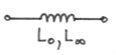
\includegraphics[width=1.5cm]{./bilder/LTyp}
			}
			& \parbox{3.2cm}{
				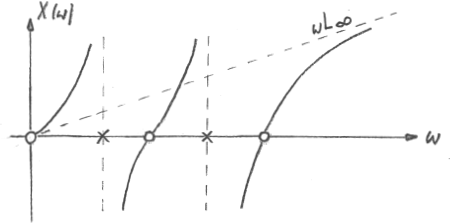
\includegraphics[width=3cm]{./bilder/RET-LTyp}
			}
			& $ \underline{Z}(p)=p\frac{a_np^{n-1}+ \ldots +a_1}{b_mp^m+ \ldots b_0}$
			& $ = \frac{\jom L_{\infty}[(\jom)^2 + \omega_3^2][\ldots]}{[(\jom)^2 +
			\omega_2^2][\ldots]}$ 
			& $ \begin{matrix}
            		\underline{Z}(p)\mid_{\rightarrow\infty}=p\frac{a_n}{b_m}=pL_{\infty}\\
            		\underline{Z}(p)\mid_{\rightarrow 0}=p\frac{a_1}{b_0}=pL_{0}
              	\end{matrix}$
			& $ \begin{matrix}
            		n: ungerade \\
            		m=n-1
                \end{matrix}$\\
		\hline
			\parbox{1.6cm}{
				C-Typ \\
				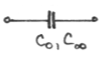
\includegraphics[width=1.5cm]{./bilder/CTyp}
			}
			& \parbox{3.2cm}{
				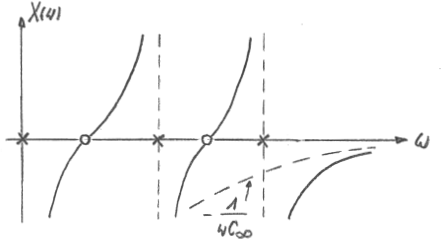
\includegraphics[width=3cm]{./bilder/RET-CTyp}
			}
			& $ \underline{Z}(p)=\frac{1}{p} \frac{a_np^{n}+ \ldots +a_0}{b_mp^{m-1}+ \ldots b_1}$
			& $ = \frac{[(\jom)^2 + \omega_2^2][\ldots]}
					{\jom C_{\infty}[(\jom)^2 + \omega_3^2][\ldots]}$ 
			& $ \begin{matrix}
					\underline{Z}(p)\mid_{\rightarrow\infty}=\frac{1}{p}\frac{a_n}{b_m}=\frac{1}{pC_{\infty}}\\
					\underline{Z}(p)\mid_{\rightarrow 0}=\frac{1}{p}\frac{a_1}{b_0}=\frac{1}{pC_{0}}
				\end{matrix}$
			& $ \begin{matrix}
					n: gerade \\
					m=n+1
				\end{matrix}$\\
		\hline
			\parbox{1.6cm}{
				P-Typ \\
				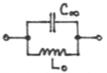
\includegraphics[width=1.5cm]{./bilder/PTyp}
			}
			& \parbox{3.2cm}{
				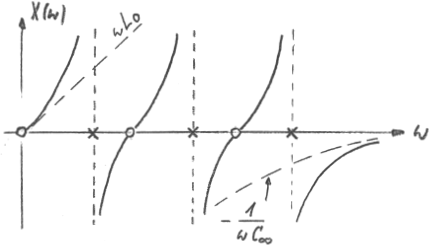
\includegraphics[width=3cm]{./bilder/RET-PTyp}
			}
			& $ \underline{Z}(p)=p\frac{a_np^{n-1}+ \ldots +a_1}{b_mp^m+ \ldots b_0}$
			& $ = \frac{\jom[(\jom)^2 + \omega_3^2][\ldots]}
					{C_{\infty}[(\jom)^2 + \omega_2^2][(\jom)^2 + \omega_4^2]\ldots]}$ 
			& $ \begin{matrix}
					\underline{Z}(p)\mid_{\rightarrow\infty}=\frac{1}{p}\frac{a_n}{b_m}=\frac{1}{pC_{\infty}}\\
					\underline{Z}(p)\mid_{\rightarrow 0}=p\frac{a_1}{b_0}=pL_{0}
				\end{matrix}$
			& $ \begin{matrix}
               		n: ungerade\\
               		m=n+1
                \end{matrix}$\\
		\hline
			\parbox{1.6cm}{
				S-Typ \\
				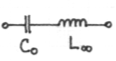
\includegraphics[width=1.5cm]{./bilder/STyp}
			}
			& \parbox{3.2cm}{
				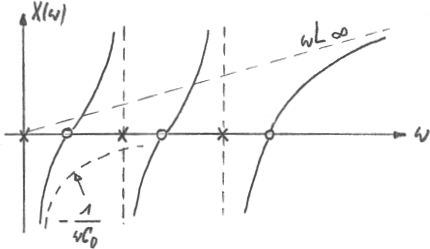
\includegraphics[width=3cm]{./bilder/RET-STyp}
			}
			& $ \underline{Z}(p)=\frac{1}{p} \frac{a_np^{n}+ \ldots +a_0}{b_mp^{m-1}+ \ldots b_1}$
			& $ = \frac{[L_{\infty}(\jom)^2 + \omega_2^2][(\jom)^2 +
				\omega_4^2][\ldots]} 
				{\jom[(\jom)^2 + \omega_3^2]\ldots]}$
			& $ \begin{matrix}
					\underline{Z}(p)\mid_{\rightarrow\infty}=p\frac{a_n}{b_m}=pL_{\infty}\\
					\underline{Z}(p)\mid_{\rightarrow 0}=\frac{1}{p}\frac{a_1}{b_0}=\frac{1}{pC_{0}}
				\end{matrix}$
			& $ \begin{matrix}
               		n: gerade\\
               		m=n-1
                \end{matrix}$\\
		\hline
	\end{tabular}
	\renewcommand{\arraystretch}{1}
\newpage		
		
\subsection{Minimalreaktanzeintor (MRET)}
	%RET in MRET wandeln:\\
	\begin{enumerate}{\setlength{\itemsep}{0cm}\setlength{\parsep}{0cm} \setlength{\topsep}{0cm}}
      \item Netzwerk übersichtlich aufzeichnen 
      \item Tor offen; Kreise suchen die nur L oder C enthalten; Ein
      Element des Kreises weglassen, es darf aber kein anderer Zweig stromlos werden. 
      \item Tor kurzgeschlossen; Trennbündel suchen(Knoten an denen nur
      L oder C liegen); Ein Element kurzschliessen, dabei darf kein anderes Element kurzgeschlossen werden.
      \item Die verbleibenden Elemente im MRET haben nicht mehr die
      gleichen Grössen und müssen neu berechnet werden.
    \end{enumerate}
	
	%Anzahl Elemente = Höchste Potenzfunktion $\underline{Z}(p)$
		
			
\subsection{Dualität}
	\begin{tabular}{ll}
    \parbox{11.5cm}{    		
			\textbf{Vorgehen}
			\begin{enumerate}{\setlength{\itemsep}{0cm}\setlength{\parsep}{0cm} \setlength{\topsep}{0cm}}
	          \item Netzwerk ohne Kreuzungen aufzeichnen
	          \item In jede Masche (auch in Umfangsmasche) einen dualen Knoten
	          setzen
	          \item Knoten von anstossenden Maschen verbinden. Jeder dieser Maschen
	          hat gemeinsamen Zweig (dualen Zweig). 
	          \item  In die dualen Zweige die dualen Schaltungselemente einsetzen.
	        \end{enumerate}
    	}
    	& \parbox{6.5cm}{
    		\begin{tabular}{c c}
            $C \leftrightarrow L$ 
            	&$R \leftrightarrow G$ \\
            $u \leftrightarrow i$
            	& $\underline{Z} \leftrightarrow \underline{Y}$ \\
            Knoten $\leftrightarrow$ Masche
            	& Stern $\leftrightarrow$ Dreieck \\
            \multicolumn{2}{c}{Parallelschaltung $\leftrightarrow$
            	Serieschaltung} \\
            \multicolumn{2}{c}{Stromquelle $\leftrightarrow$ Spannungsquelle}            
	        \end{tabular}
			\vspace{.1cm} 

			\textbf{Zahlenwerte der Dual-Elemente}\\
			\begin{minipage}{2cm}
	        	$R'=D^2G$ \\
	        	$L'=D^2C$
	        \end{minipage}
			\begin{minipage}{2cm}
	        	$C'=\frac{L}{D^2}$ \\
	        	$G'=\frac{R}{D^2}$
	        \end{minipage}
			\begin{minipage}{2cm}
	        	$U'=DI$ \\
	        	$I'=\frac{U}{D}$
	        \end{minipage}
			\begin{minipage}{4cm}
	        	$D =$Dualfaktor $[\Omega]$
	        \end{minipage}
			\vspace{.1cm} 

    		\textbf{Impedanzfunktion}
    		$Z_D(s) = \frac{1}{Z_(s)}$ \\
    	}
    \end{tabular}

\subsection{Netzwerksynthese}
	\begin{tabular}{ll}
    	\parbox{9cm}{
			\textbf{Mittels Partialbruchzerlegung}
				\begin{enumerate}{\setlength{\itemsep}{0cm}\setlength{\parsep}{0cm} \setlength{\topsep}{0cm}}
		          \item $j\omega \Rightarrow p$\\
		          $F(p)=\frac{2p^6+22p^4+68^2+48}{3p^5+21p^3+30p}$
		          \item $F(p)$ Ausdividieren, falls $n>m$
		          \item Nenner des echten Bruches zerlegen und \\
		          Ansatz bilden\\
		          $\frac{2}{3}p+\frac{8p^4+48p^2+48}{3p^5+21p^3+30p}=\frac{A}{3p}+\frac{Bp}{p^2+2}+\frac{Cp}{p^2+5}$
		          \item Erweitern und Koeffizienten bestimmen\\
		          $A=\frac{24}{5} \qquad B=\frac{8}{9} \qquad C=\frac{8}{45}$
		          \item Koeffizienten einsetzen\\
		          $F(p)=\frac{2}{3}p+\frac{1}{\frac{15}{24}p}+\frac{1}{\frac{9}{8}p+\frac{1}{\frac{4}{9}p}}+\frac{1}{\frac{45}{8}p+\frac{1}{\frac{8}{255}p}}$
		          \item Schaltung aufzeichnen:\\
		          (Schaltung ist MRET!)
                \end{enumerate}
        }
    	\parbox{9cm}{
			\textbf{Mittels Kettenbruchzerlegung}
				\begin{enumerate}{\setlength{\itemsep}{0cm}\setlength{\parsep}{0cm} \setlength{\topsep}{0cm}}
                  \item $j\omega \Rightarrow p$\\
                  $F(p)=\frac{2p^6+22p^4+68p^2+48}{3p^5+21p^3+30p}$
		          \item $F(p)$ ausdividieren\\
		          $=\frac{2}{3}p+\frac{8p^4+48p^2+48}{3p^5+21p^3+30p}$
		          \item Kehrwert des Restes wieder ausdividieren\\
		          $\frac{2}{3}p+\frac{1}{\frac{3p^5+21p^3+30p}{8p^4+48p^2+48}}=\frac{2}{3}p+\frac{1}{\frac{3}{8}p+\frac{3p^3+12p}{8p^4+48p^2+48}}$
		          \item Schritt zwei wiederholen bis kein Rest mehr\\
		          vorhanden ist\\
		          $F(P)=\frac{2}{3}p+\frac{1}{\frac{3}{8}p+\frac{1}{\frac{8}{3}p+\frac{1}{\frac{3}{16}p+\frac{1}{\frac{16}{3}p+\frac{1}{\frac{1}{16}p}}}}}$
		          \item Schaltung aufzeichnen:
                \end{enumerate}
         }
	\end{tabular}\\

	\begin{tabular}{cc}
    	\begin{minipage}{9cm}
        	Impedanzfunktion $Z(p)$:\\
            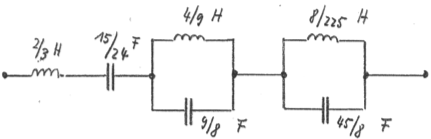
\includegraphics[width=6cm]{./bilder/PartialbruchImpedanzfunktion}
        \end{minipage}

		\begin{minipage}{9cm}	
        	Impedanzfunktion $Z(p)$:\\
            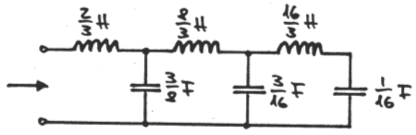
\includegraphics[width=6cm]{./bilder/KettenbruchImpedanzfunktion}
        \end{minipage}
\\
		\begin{minipage}{9cm}
        	Admittanzfunktion $Y(p)$:\\
            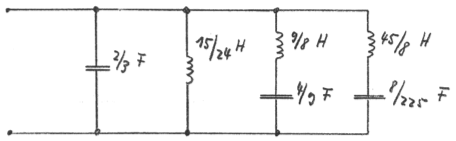
\includegraphics[width=6cm]{./bilder/PartialbruchAdmittanzfunktion}
        \end{minipage}

		\begin{minipage}{9cm}
        	Admittanzfunktion $Y(p)$:\\
            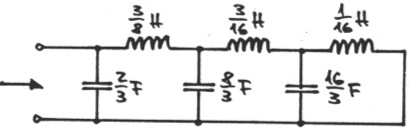
\includegraphics[width=6cm]{./bilder/KettenbruchAdmittanzfunktion}
        \end{minipage}
    \end{tabular}

